\documentclass[letterpaper,twoside,12pt]{article}
\usepackage{graphicx}
\usepackage[margin=0.8in]{geometry}


\title{ER2201 Session Delay Closures}
%\author[1]{L. Benkevitch}

\begin{document}

\maketitle

The figures below show closure delay distributions over 5.5 hours and histograms of absolute magnitudes for the multi-band and single-band delays and their residuals.

The closure delay calculations of the total multi-band and single-band delays (the two last Figs.) obviously fail.

\begin{figure}[h!]
  %\begin{center}
  \centering
  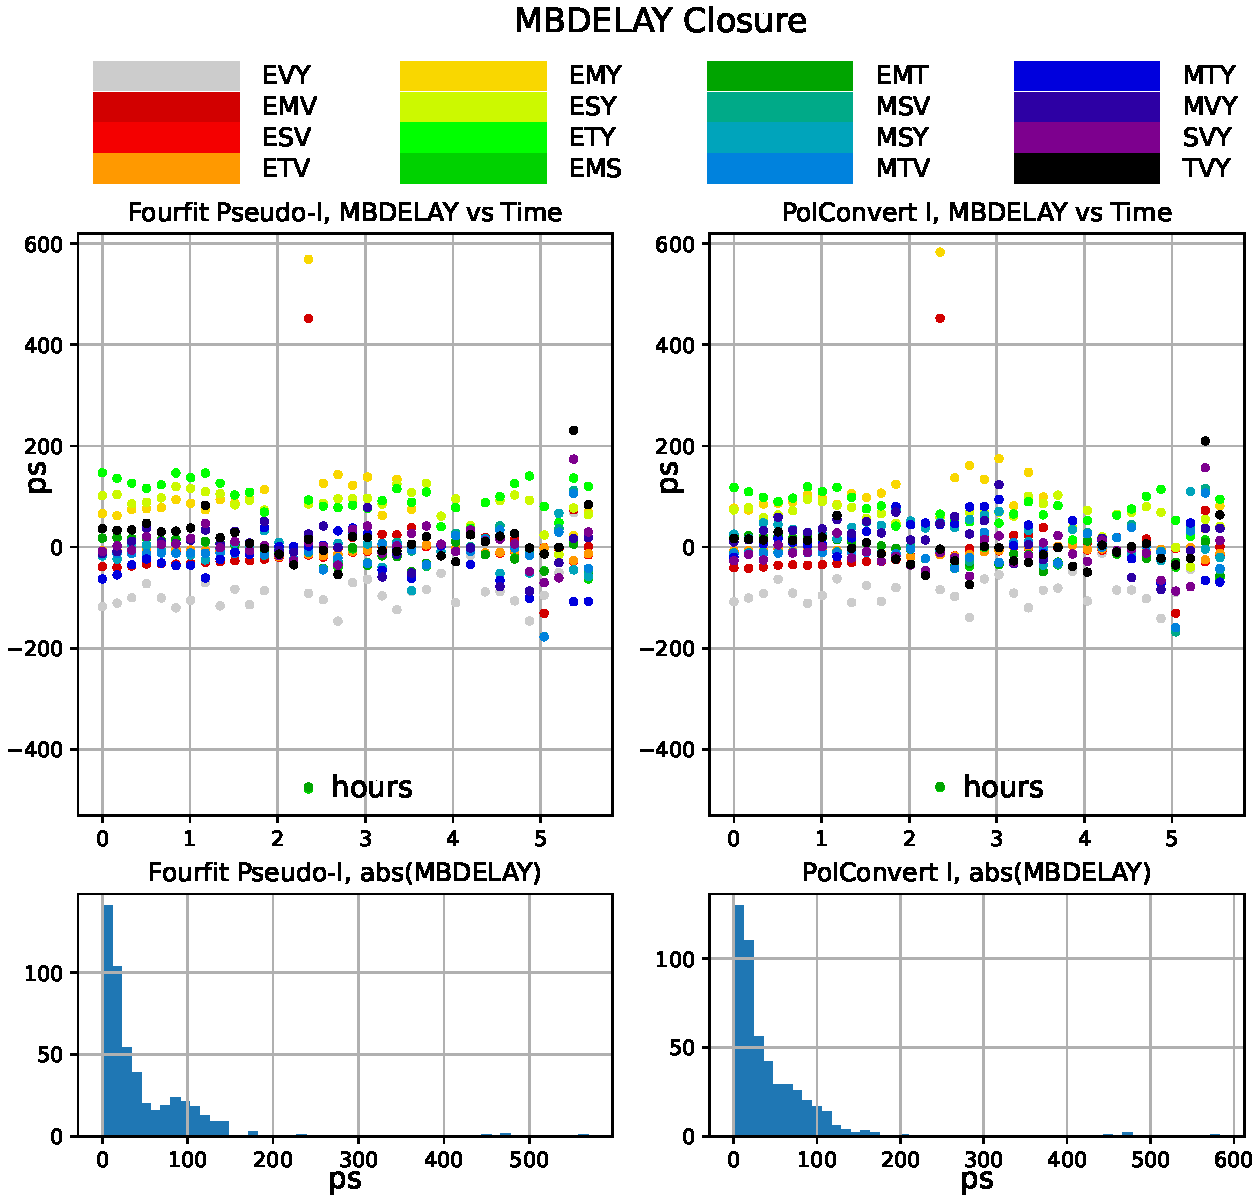
\includegraphics[width=35pc]{MBDELAY_Closure_Delay.pdf}
  \caption{\small MBDELAY closure delay distributions over 5.5 hours and histograms of their absolute magnitudes.}
  \label{mbd}
  %\end{center}
\end{figure}


\begin{figure}[ht!]
  \begin{center}
  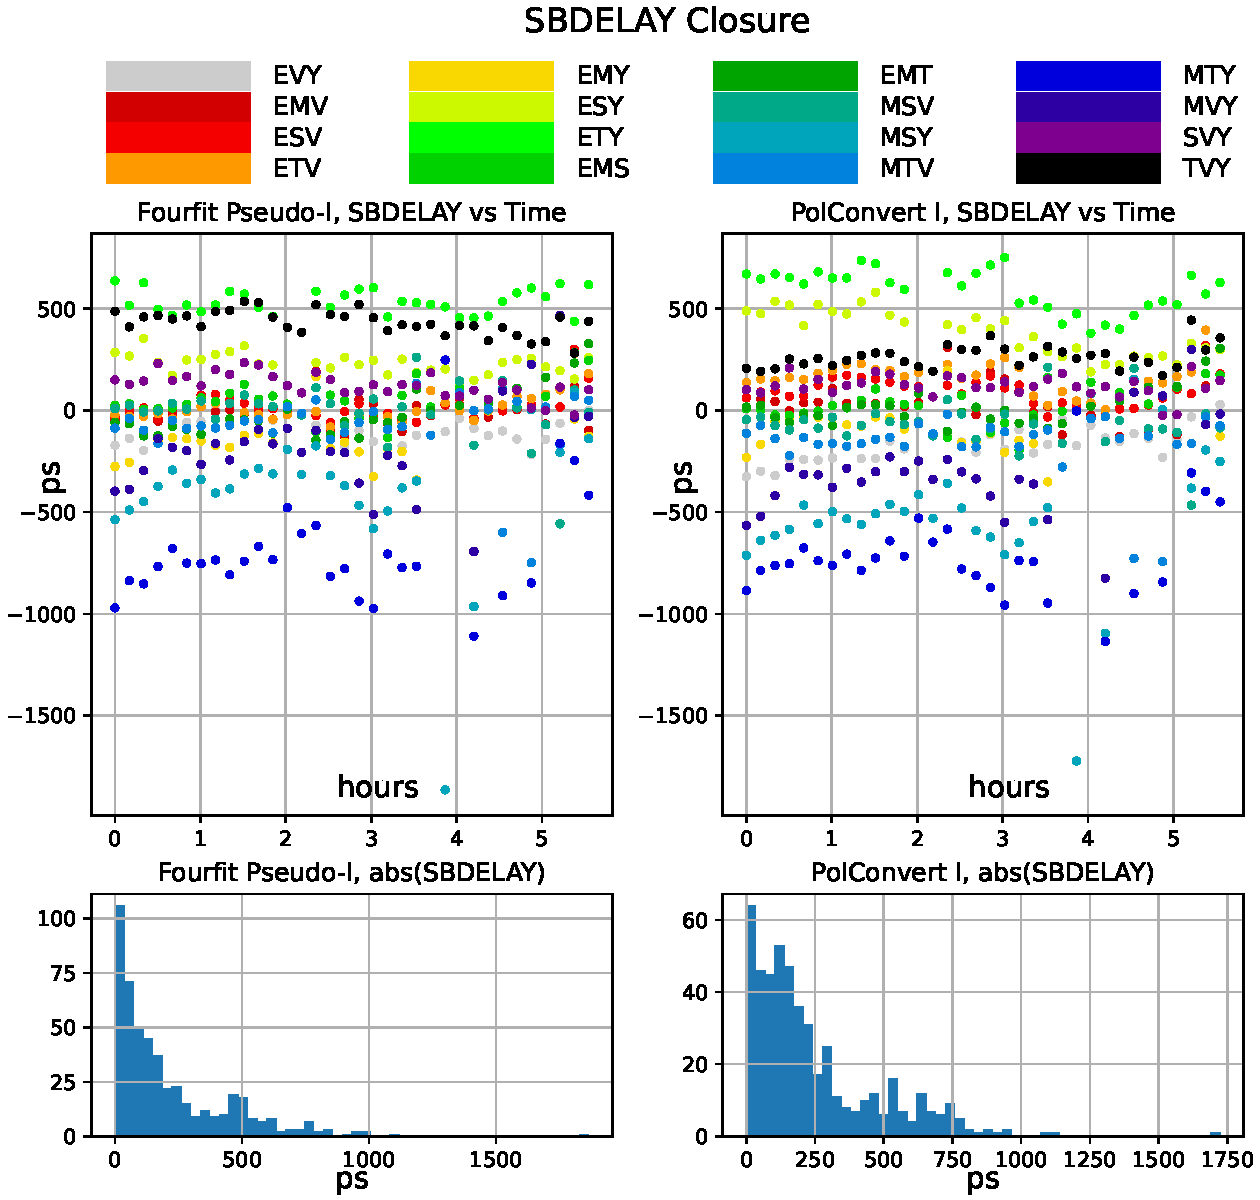
\includegraphics[width=40pc]{SBDELAY_Closure_Delay.pdf}
  \caption{\small SBDELAY closure delay distributions over 5.5 hours and histograms of their absolute magnitudes.}
  \label{sbd}
  \end{center}
\end{figure}


\begin{figure}[ht!]
  \begin{center}
  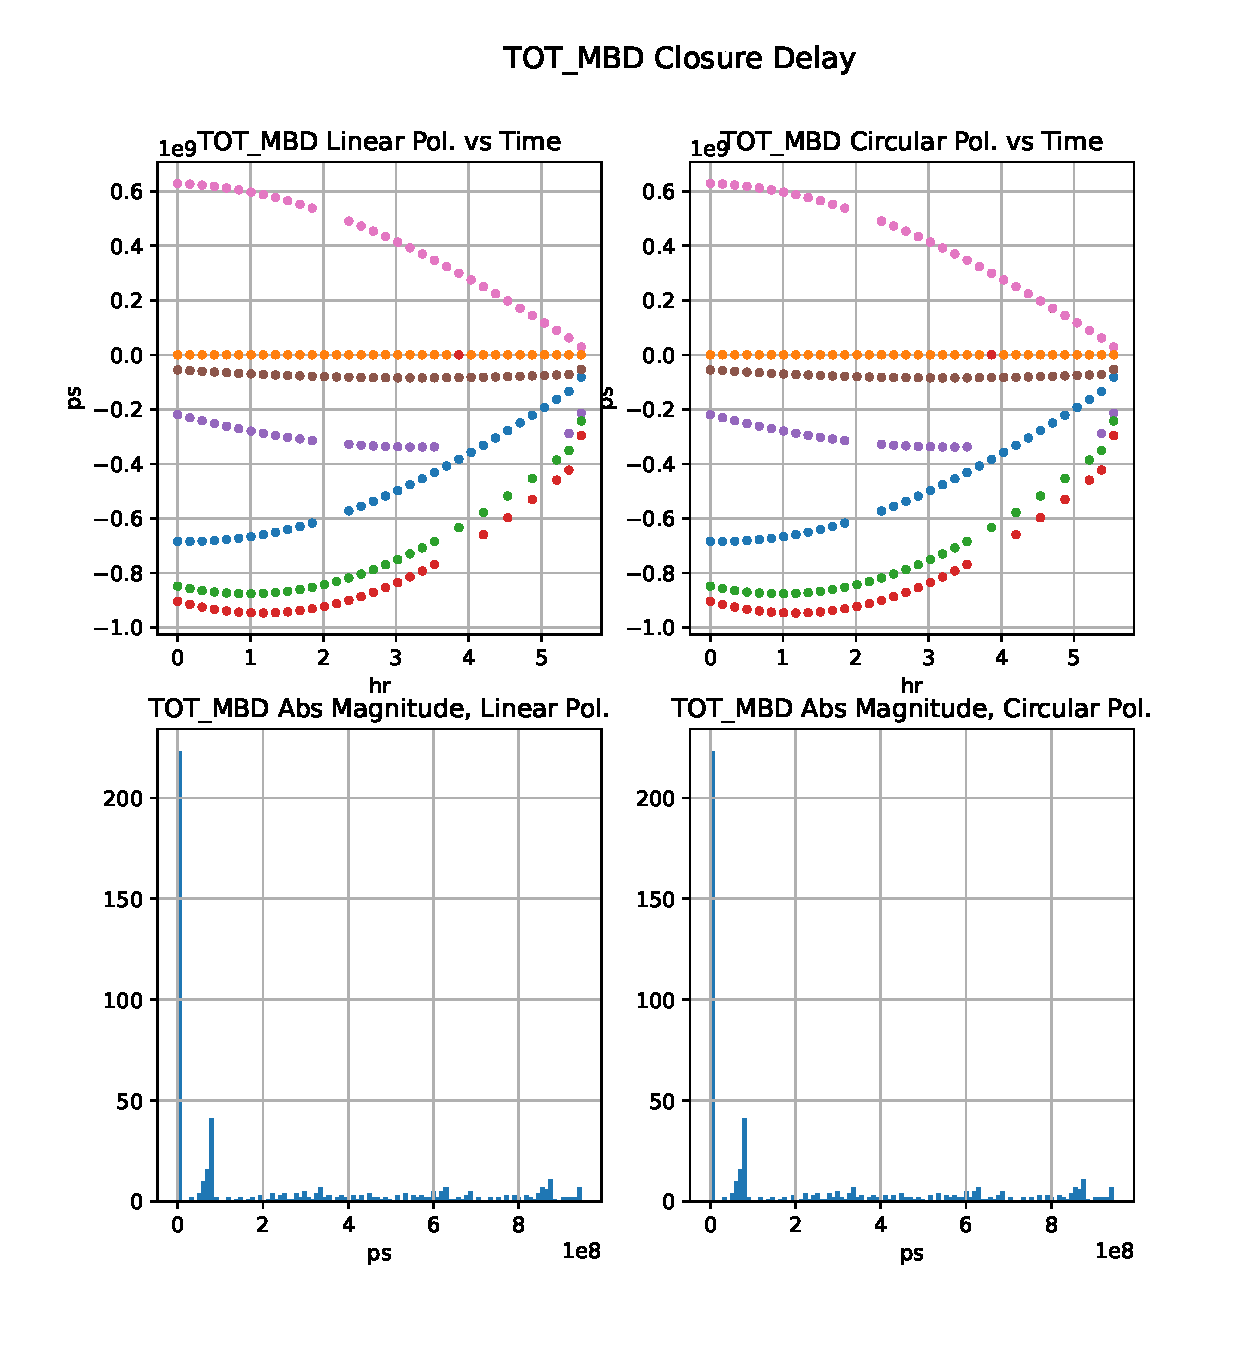
\includegraphics[width=40pc]{TOT_MBD_Closure_Delay.pdf}
  \caption{\small Total MBDELAY closure delay distributions over 5.5 hours and histograms of their absolute magnitudes.}
  \label{tot_mbd}
  \end{center}
\end{figure}


\begin{figure}[ht!]
  \begin{center}
  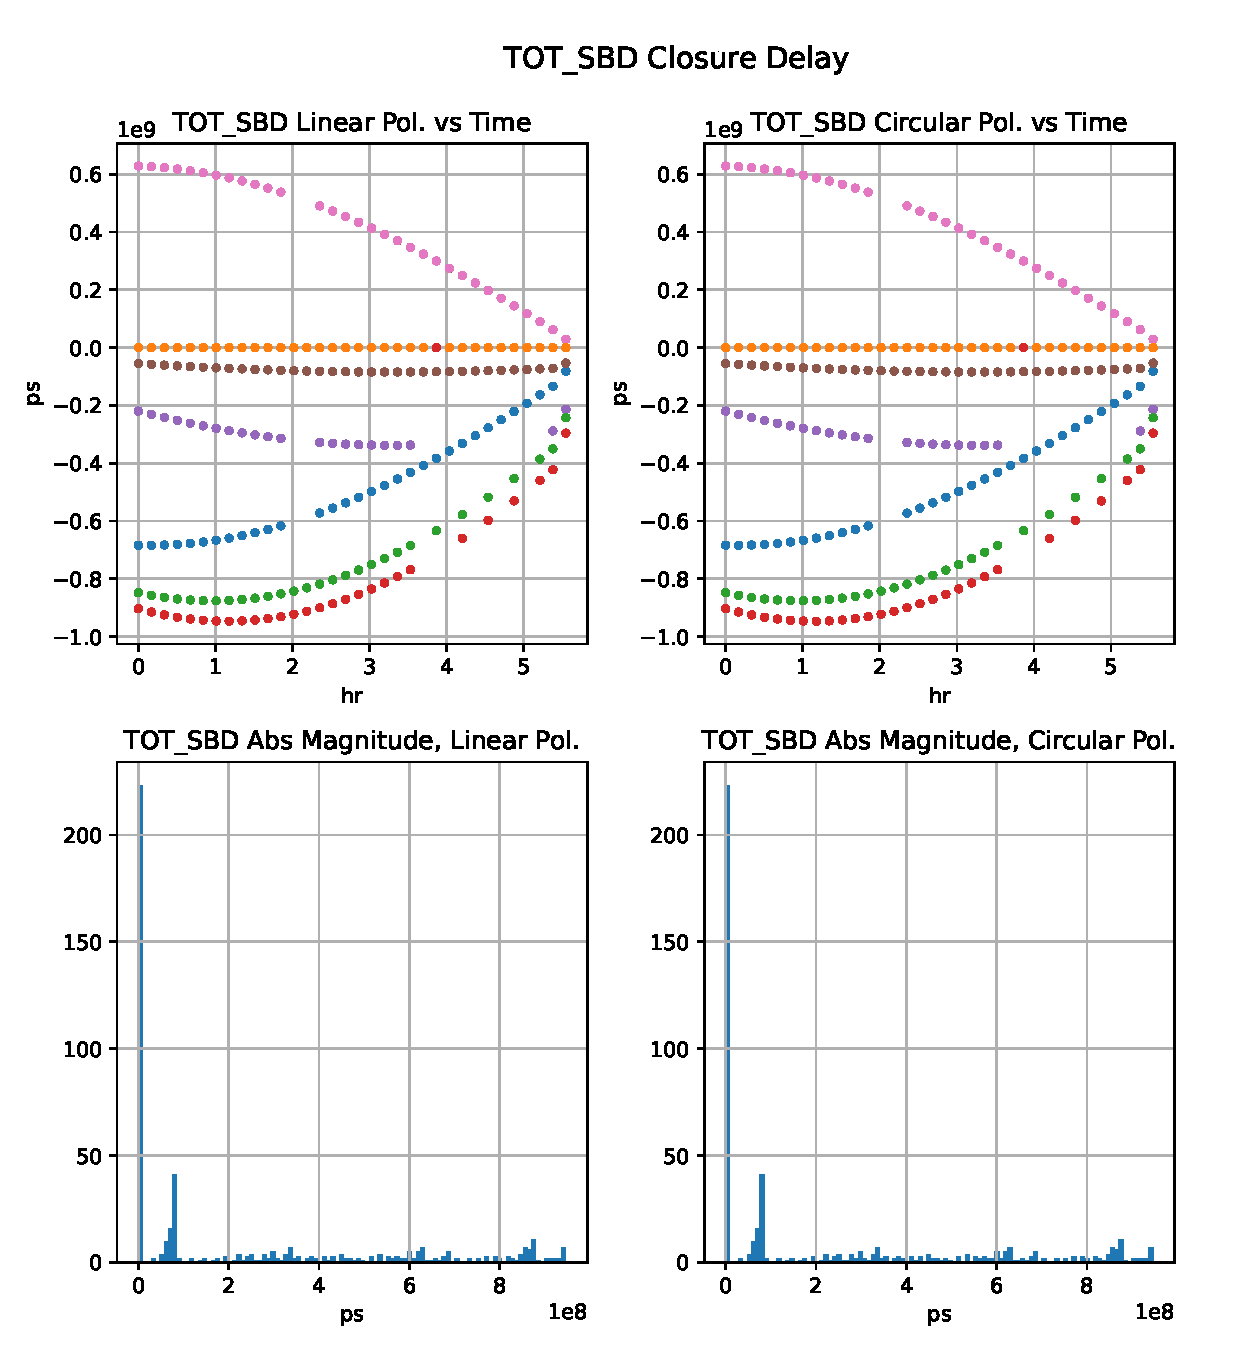
\includegraphics[width=40pc]{TOT_SBD_Closure_Delay.pdf}
  \caption{\small Total SBDELAY closure delay distributions over 5.5 hours and histograms of their absolute magnitudes.}
  \label{tot_mbd}
  \end{center}
\end{figure}




\end{document}








